\chapter{Preparation}

%\section{Background}

\section{Graph representational learning}
\label{sec:GRL}

% Formal definition of graph based data

%% Formal definition of a graph

A \emph{graph} can be formally represented as the tuple $\gG(\sV, \sE, \mX)$ where $\sV$ is the set of nodes in the graph, $\sE$ is the set of edges, and $\mX$ the data associated with the graph also known as the input features.
Two nodes of the graph, $v_i, v_j \in \sV$, are \emph{connected} if and only if $(v_i, v_j) \in \sE$, the edge is directed with $v_i$ as the source and $v_j$ as the destination.
%It is possible to associate data with the edges of the graph where $(v_i, v_j, \textbf{e}_{ij}) \in \sE$ represents a connection between $v_i$ and $v_j$ and associated vector $\textbf{e}_{ij}$.
Each node, $v_i \in \sV$, has associated data represented by the \emph{feature vector} $\vx_i = \emX_{i,\star}$ the $i^{th}$ row of $\mX$.

The edges can be represented as an \emph{adjacency matrix}, $\mA$, where 
\begin{equation}
    \label{eq:adj}
    \emA_{ij} = \begin{cases}1 &\text{iff $(v_i, v_j) \in \sE$} \\ 0 &\text{otherwise}\end{cases}.
\end{equation}
This allows the edge information to be utilised by a NN along with the features $\mX$.
Furthermore, each node, $v_i \in \sV$, has \emph{neighbours} which is set of connected nodes,
\begin{equation}
    \label{eq:neighbour}
    \sN_i = \{v_j | (v_i, v_j) \in \sE \vee (v_j, v_i) \in \sE\},
\end{equation}
where element of $\sN_i$ is considered a \emph{neighbour} of the node $v_i$.
%For ease of writing $\mX_{\sN_i}$ represents the features of the neighbours of $v_i$ defined as 
%\begin{equation}
%    \label{eq:neighbour-reps}
%    \mX_{\sN_i} = \{\{\vx_j | v_j \in \sN_i\}\}.\footnote{As the neighbours may have the same feature vector this must be a multiset.}
%\end{equation}
%If there is data associated with the edges, such as edge weights, this value is stored in the adjacency matrix.
%An unweighted graph can be described as a weighted graph with edge weights of value $1$.
%Adjacency matrices can be very sparse, meaning they have very few non-zero values, and therefore the matrix is commonly stored in a \emph{coordinate matrix} (COO) of size $2 \times N$ for $N$ edges in the graph thus only storing edge information.

% Formal definition of representational learning

The goal of \emph{graph representational learning} is to find, for each $v_i \in \sV$, a vector $\vh_i^{(l)}$ based on the the input features $\mX$ and adjacency matrix $\mA$, where $\vh_i^{(0)} = \vx_i$.
$\vh_i^{(l)}$ is lnown as the \emph{node representation} after the $l^{th}$-layer and $\mH^{(l)}$ is the total graph representation where $\mH_{i, \star}^{(l)} = \vh_i^{(l)}$.
%It is therefore important to consider an updated version of equation \ref{eq:neighbour-reps} as $mH_{\sN_i}^{(l)} = \{\{\vh_j^{(l)} | v_j \in \sN_i\}\}$ however $\mX_{\sN_i}$ will be used and the

% Comparison of graph, edge and node based learning

%% Expand the above definition to edges and graphs
%% discussion of edge weights in training when talking about edge learning
%% discussion of pooling functions with graph classification

These representations may then be used as input to a classifier to solve one of 3 different classification tasks: node classification, graph classification, link prediction.
This project focuses on node classification, where each node is assigned a label, and graph classification, where the graph as a whole is assigned a label.
%Node classification classifies each node solely on the final node representation $\vh_i$.
%Comparitively graph classification aggregates all of the node representations and classifies the entire graph accordingly.

\subsection{Graph neural networks}

%% Formal definition of a function on this graph
%%      Think about Petars talk here

%% The idea of invariants, equivariants and approaches

The updated node representations should depend on the local neighbourhood of each node.
If the same local neighbourhood representations were to be permuted the updated representation should remain the same as the neighbourhood topology is the same.
Therefore consider a vector valued function, $\vf$, taking neighbourhood representations, $\mX_{\sN_i}$, and adjacency matrix, $\mA$, and producing a neighbourhood representation $\vf(\mX_{\sN_i}, \mA)$.
Given some permutation, $\mP$, $\vf(\mP\mX_{\sN_i}, \mP\mA\mP^T) \equiv \vf(\mX_{\sN_i}, \mA)$.\footnote{As the rows and columns of the adjacency matrix must be permuted the permutation matrix is applied twice, with the premultiplication transposed to permute the columns.}

Furthermore, if the node features are permutated then the updated node representations should be as well.
Thus consider a matrix valued function, $F$, taking the input representations and adjacency matrix, and producing a new representation matrix.
It must be the case that $F(\mP\mX, \mP\mA\mP^T) \equiv \mP F(\mX, \mA)$.

For the node representation update function, $F$, to be equivarient it suffices for the neighbourhood representation function to be invariant, \Aref{app:perm}.
For the neighbourhood representation to be invariant an invariant aggregation function, $\bigoplus$, combines updated neighbourhood representations.
Thus a neighbour representation\footnote{Multiple formulations exist and is an area of active research.} for $\vx_i$ is $\bigoplus_{\vx_j \in \mX_{\sN_i}}c_{ij}\bm{\psi(\vx_j)}$.
Where $\bm{\psi}$ is an individual node representation update function.
This leads to a general invariant node representation update function

\begin{equation}
    \label{eq:conv-def}
    \bm{\phi}(\vx_i, \mX_{\sN_i}) = \bm{\varphi}(\vx_i, \bigoplus_{\vx_j \in \mX_{\sN_i}}c_{ij}\bm{\psi}(\vx_j)).
\end{equation}

%This function can be described by a function, $f$, which acts on a single node, $v_i$, using the feature vector, $\vx_i$, and neighbours, $\sN_i$.
%Rather than $f$ being applied to the input features consider some node representation $\vh_i^{(l)}$ after $l$ iterations, where $\vh_i^0 = \vx_i$.
%Then $\vh_i^{(l+1)} = f^{(l)}(\vh_i^{(l)}, \sN_i)$, where $f^{(l)}$ is the $l^{th}$ application of the function $f$.

% Formal definition of a graph neural network

%% Expand on the invariants and equivariants above (maybe only start that here)
%% Formalise the notion of how a GNN would behave
%% Discuss the differing approaches

% Potentially the motivation behind this formalisation

%% This is the invariance and equivariance
%% Might be possible to motivate this from the development perspective

% Identify the root of deep learning in its formulation

%% Highlight the concept of non-linear layers
%% potentially a brief discussion on the importance of this concept

\subsection{Graph convolutional network}
\label{sec:GCN}

% Formal implementation of Graph Convolutional Network

%% Expand on the convolutional approach to discuss this formulation

\subsubsection{As a GNN}

The GCN is the simplest implementation of the formulation outlined above.
The principle is to add the edge weighted sum of a node's neighbour representations to the current node representation.
This maintainsd the invariance constraint but nodes with a high degree are overly represented and so each term is normalised by the degree of the connecting nodes.
This results in the common representation of GCN as

\begin{equation}
    \label{eq:GCN-as-GNN}
    f(\vh_i^{(l)}, \mA) = \frac1{d_i + 1}\vh_i^{(l)} + \sum_j^N\frac{\emA_{ij}}{\sqrt{(d_i + 1)(d_j + 1)}}\vh_j^{(l)},
\end{equation}
\begin{equation}
    \vh_i^{(l+1)} = \sigma(f(\vh_i^{(l)}, \mA)\theta_i^{(l)})
\end{equation}

where $d_i = \sum_j^N \emA_{i,j}$ (the degree of node $v_i$), $\theta_i^{(l)}$ is a learnable parameter, and $\sigma$ is an activation function. Comparing to equation \ref{eq:conv-def} $c_{ij} = \frac1{\sqrt{(d_i + 1)(d_j + 1)}}$ and $\sum_j^N$ is equivalent to $\bigoplus_{\vx_j \in \mX_{\sN_i}}$. 

%\begin{align*}
%    &\vx_j \in \mX_{\sN_i} \\
%    \iff &j \in \sN_i &&\text{by def. \ref{eq:neighbour-reps}} \\
%    \iff &(v_i, v_j) \in \sE \vee (v_j, v_i) \in \sE &&\text{by def. \ref{eq:neighbour}} \\
%    \iff &A_{ij} = 1 &&\text{by def. \ref{eq:adj}}
%\end{align*}

%To better demonstrate that the same operation is being applied to each neighbouring representation (including the nodes current representation) 
equation \ref{eq:GCN-as-GNN} may be rewritten as

\begin{equation}
    \label{eq:same-op}
    f(\vh_i^{(l)}, \mA) = (d_i + 1)^{-\frac12}1(d_i + 1)^{-\frac12}\vh_i^{(l)} + \sum_j^N(d_i + 1)^{-\frac12}\emA_{ij}(d_i + 1)^{-\frac12}\vh_j^{(l)}.
\end{equation}

Let $\mD$ be the degree matrix, $\emD_{ii} = \sum_j^N \emA_{ij}$, and $\mH^{(l)}$ the node representations of the graph after layer $l$. Equation \ref{eq:same-op} is therefore

\begin{equation}
    F(\mH^{(l)}, \mA) = (\mD + \mI)^{-\frac12}(\mA + \mI)(\mD + \mI)^{-\frac12}\mH^{(l)}.
\end{equation}

Let $\widetilde{\mA} = \mA + \mI$, then $\widetilde{\emD}_{ii} = \sum_j^N \widetilde{\emA}_{ij} = \sum_j^N [\emA_{ij} + 1] = \emD_{ii} + 1$ thus $\widetilde{\mD} = \mD + \mI$.
This reformulation gives the following graph operator 
\begin{equation}
    \label{eq:op}
    \mS = \widetilde{\mD}^{-\frac12}\widetilde{\mA}\widetilde{\mD}^{-\frac12}.
\end{equation}

Thus a GCN layer can be interpretted as a graph operator and non-linearity, giving
\begin{align}
    \label{eq:GCN1}
    \mH^{(l+1)} & = \sigma(\mS\mH^{(l)}\bm{\Theta}^{(l)})
\end{align}
%resulting in the following formulation
%\begin{equation}
%    F(\mH^{(l)}, \mA) = \mS\mH.
%\end{equation}

%The function is parameterised by a weight matrix, $\bm{\Theta}$, to give a single layer 

\subsubsection{As a convolution}
\label{sec:conv}

To motivate the idea of the SGC it is important to think of $\mS$ from a different perspective, as a graph convolution filter. A convolution is a multiplication of two functions, in this case a signal,\footnote{The signal is a function $\vh : \sV \to \R^n$ however as the nodes are fixed each signal can be represented as a vector using the notation $\vh_i \equiv \vh(v_i)$.}
represented by the node representation $\vh_i \in \R^n$, and a filter, $f_\theta$ paramaterised by $\theta$.

As an analogy to Fourier analysis $f_\theta \star_\sG \vh_i$ is defined in the graph spectral domain.
Any signal on a graph can be projected onto the eigenvectors of the graph Laplacian, $\mL = \mU\bm{\Lambda}\mU^T$, where $\bm{\Lambda} = \operatorname{diag}(\lambda_0, ..., \lambda_{n-1})$.
Therefore the graph Fourier transform of the signal is
\begin{align}
    \hat{\vh_i} &= \mU^T\vh_i, \\
    \hat{f_\theta} &= \mU^Tf_\theta.
\end{align}

%As an analogy to classical Fourier analysis the operation is defined in the spectral domain of the graph allowing for the convolution to be a pointwise product.
%
%Let $\mL$ be the graph Laplacian with eigendecomposition $\mU\bm{\Lambda}\mU^T$ where $\bm{\Lambda} = \operatorname{diag}(\lambda_0, ..., \lambda_{n-1})$. Define $\hat{\vh_i}$, the graph Fourier transform of the signal, as
%\begin{equation}
%    \label{eq:graph-fourier}
%    \hat{\vh_i} = \mU^T\vh_i.
%\end{equation}

%Equation \ref{eq:graph-fourier} carries out the dot product between $\vh_i$ and each of the eigenvectors of the graph Laplacian, $\mL$.
%This corresponds to the ``frequency'' of the signal $\vh_i$ with respect to the frequencies of the graph.
%This transforms $\vh_i$ into its frequency components according to the spectral domain of the graph.

$\hat\vh_i$ and $\hat f_\theta$ are now both projected onto the graph eigenvectors.
As the eigenvectors are orthonormal (\Aref{app:laplacian}) this means $\mU^T(f_\theta \star_\sG \vh_i) = \hat f_\theta \odot \hat\vh_i$ where $\odot$ is the hadamard product.
Let $\hat\mF_\theta = \operatorname{diag}(f_\theta)$ then
\begin{equation}
    f_\theta \star_\sG \vh_i = \mU\hat\mF_\theta\mU^T\vh_i.
\end{equation}

%followed by an inverse graph Fourier transform. To simplify the equation define 
%\begin{equation}
%    \label{eq:filter1}
%    \hat\mF_{\bm{\theta}} = \operatorname{diag}\hat f_\theta = \operatorname{diag}{\bm{\theta}}
%\end{equation}
%where $\bm{\theta}$ is a vector of parameters which can be learnt by a NN. Resulting in the following formalisation of a graph convolution
%\begin{equation}
%    \label{eq:graph-conv}
%    f_\theta *_\sG \vh_i = \mU\hat\mF_{\bm{\theta}}\mU^T\vh_i.
%\end{equation}

To prevent $\hat\mF_\theta$ growing with the dimension of the signal it can be defined as a power series of the fixed Laplacian eigenvalue matrix,
\begin{equation}
    \label{eq:filter}
    \hat\mF_{\bm{\theta}} = \sum_{i=0}^k\theta_j\bm{\Lambda}^j.
\end{equation}

\textit{Kipf et al.}\cite{kipf2016semi} suggest using $k=1$ and define $\theta = \theta_0 = -\theta_1$. The resulting graph convolution is
\begin{equation}
    \label{eq:GCN-comp}
    f_\theta *_\sG \vh_i = \sum_{j=0}^1\theta_j(\mU\bm{\Lambda}\mU^T)^j\vh_i = \theta(\mI - \mL)\vh_i.\footnote{$\mU\bm{\Lambda}^j\mU^T = \mU\underbrace{\bm{\Lambda}\cdots\bm{\Lambda}}_j\mU^T = \underbrace{\mU\bm{\Lambda}\mU^T\mU\cdots\mU^T\mU\bm{\Lambda}\mU^T}_j = (\mU\bm{\Lambda}\mU^T)^j$}
\end{equation}

Computation of the eigendecomposition of $\mL$ is expensive for large graphs so \textit{Hammond et al.}\cite{hammond2011wavelets} suggest using Chebyshev polynomials (\Aref{app:chebyshev}).
%With the additional assumption that a NN can adapt to scaling we assume that the maximum eigenvalue is approximately $2$.
Using the first order Chebyshev polynomial, $\mL - \mI$,
and the normalised graph Laplacian, $\mL = \mI - \mD^{-\frac12}\mA\mD^{-\frac12}$ (\Aref{app:laplacian}), equation \ref{eq:GCN-comp} can be written as 
\begin{equation}
    \label{eq:no-norm}
    f_\theta *_\sG \vh_i \approx \theta(\mI - (\mL - \mI))\vh_i = \theta(\mI + \mD^{-\frac12}\mA\mD^{-\frac12})\vh_i.
\end{equation}

The filter can then be used to update the node representations as such
%Applying an individual paramaterised filter to each signal, that is each node, in the graph results in the following formulisation
\begin{equation}
    \label{eq:GCN2}
    \mH^{(l+1)} = \sigma((\mI + \mD^{-\frac12}\mA\mD^{-\frac12})\mH^{(l)}\bm{\Theta}^{(l)})
\end{equation}

To reduce the size of eigenvalues, and thus vanishing/exploding gradients, \textit{Kipf et al.}\cite{kipf2016semi} apply the following renormalisation to equation \ref{eq:no-norm} 
\begin{equation}
    \label{eq:norm}
    \mI + \mD^{-\frac12}\mA\mD^{-\frac12} \to \widetilde{\mD}^{-\frac12}\widetilde{\mA}\widetilde{\mD}^{-\frac12} = \mS.
\end{equation}

This renormalisation matches the graph operator in equation \ref{eq:op} demonstrating that GCN behaves as a graph filter.
If either formulation is used for node classification a linear classifier is appended to the computation resulting in 
\begin{equation}
    \label{eq:cls}
    \hat\mY = \operatorname{softmax}(\mS\mH^{(k-1)}\bm{\Theta}^{(k)}).
\end{equation}


%= \widetilde{\textbf{D}}^{-\frac12}\widetilde{\mA}\widetilde{\textbf{D}}^{-\frac12}\mX\textbf{\Theta}$

% Link to the paper

%% Lay out the exact formulation from the paper
%% Explain this formulation
%% include the motivations/reasonings from the paper

% Discussion of importance in the field?

%% Description of the fact that this is the first graph approach
%% Maybe a link to DeepSet

\subsection{Simplified graph convolution}
\label{sec:SGC}

% Motivation behind SGC

%% Reiterate the points made in the introduction
%% Now specifically highlight these areas in the GCN formulisation

As both approaches in \Sref{sec:GCN} demonstrate a GCN can be broken down into individual layers, containing a linear graph operation on the current node representations, stacked together using a non-linear activation function.
This means that the $k^{th}$-layer node representation requires the calculation of all the non-linear activations up until this layer.
This is apparent when looking at the formulation in equation \ref{eq:GCN1}.

\paragraph{Linearization.}
Considering the linear graph operation as a spectral filter as described in equation \ref{eq:norm} the non-linearity between layers may be considered non-critical to GCN performance.
Instead the benefit comes from the local averaging from successive filter applications as hypothesised by \textit{Wu et al.}.
%\textit{Wu et al.}\cite{wu2019simplifying} consider this hypothesis citing the benefit arises from the local averaging as apparent in the graph operation formulation described in \Sref{sec:conv}.
%The resulting model is therefore a linear multiplication of the normalised spectral filters and parameter matrix.
Removing the non-linear activation functions from equation \ref{eq:cls} results in
\begin{equation}
    \hat\mY = \operatorname{softmax}(\underbrace{\mS\cdots\mS}_k\mX\underbrace{\bm{\Theta}^{(1)}\cdots\bm{\Theta}^{(k)}}_k),
\end{equation}
where the filter is applied $k$ times to allow for the retention of the receptive field.
As $\bm{\Theta}^{(i)}$ is a learnable parameter the model may instead learn a single parameters
\begin{equation}
    \label{eq:theta}
    \bm{\Theta} = \underbrace{\bm{\Theta}^{(1)}\cdots\bm{\Theta}^{(k)}}_k.
\end{equation}
The final linearised model, SGC, is therefore
\begin{equation}
    \label{eq:SGC}
    \hat\mY = \operatorname{softmax}(\mS^{k}\mX\bm{\Theta}).
\end{equation}

As $\mS$ is fixed for a specific graph $\mS^k\mX$ is also fixed if $\mX$ is fixed.
Thus SGC can be broken down into representation extraction, $\bar\mX = \mS^k\mX$, and a classification, $\hat\mY = \operatorname{softmax}(\bar\mX\bm{\Theta})$.
This allows for $\bar\mX$ to be precomputed for node features $\mX$ or just $\mS^k$, allowing for the pre-computation of different node features.
%Furthermore, different node features can be quickly calculated as $\mS^k$ can be precomputed.

Rather than considering how many layers an SGC model has the equivalent notion of \emph{degree} is used where the degree is the power of $\mS$.
This directly corresponds to the receptive field of the model where a $k$-degree SGC model has the same receptive field as a $k$-layer GCN model.

\paragraph{Drawbacks}
SGC suffers from vanishing/exploding values in $\bm{\Theta}$ and over-smoothing\footnote{where the node representations become increasingly uniform as the increased receptive field of the model results in a global averaging of the graphs nodes.}.
\textit{Para et al.}\note{citation needed} also state that SGC has a fixed feature extraction step preventing influence on intermediate node representations.
These drawbacks motivate the extensions presented in \Sref{sec:extensions-imp} and \Sref{sec:extension-eval}.

%The fomulation in equation \ref{GCN-as-GNN} highlights that at after each layer each node representation includes a representation of its immediate neighbours.
%This means that the $k^{th}$-layer node representations are influenced by the node representations at most $k$-hops away. 

% Demonstration of how the GCN leads to the SGC

%% Demonstrate that the removal of layers logically leads to SGC
%% Explanation of how the weight matrix would behave
%% Potential hint or discussion about the effect of weight decay later

\section{Explainability}

% Overview of the concept of explainability

%% This needs some proper reading in the topic see below

% This probably requires reading some papers "yay"

NNs are presented as black-box models where the decision process used to infer an output based on input is opaque to a user.
This results in mistrust in NNs especially deep NNs where the relationship between input and output is complex.

the goal of explainability is to provide a human interpretable representation of the models decision process in inferring a specific output.
Ideally global explanations are provided allowing insight into the models full decision process rather than for a specific input.

The proposed approach to explainability that this dissertation choses is that of concepts as these can be inferred after training and thus do not effect model performance.
Furthermore, as GNNs utilise both graph structure and node features concepts can provide a better human interpretable representation of a GNNs decision process.

\subsection{Concepts}

% Explanation of what a concept is generally

%% Again this requires proper reading in the subject see above

A concept can be considered an ``interpretable'' high-level units which are more understandable to a human than the standard input units such as inidividual features, pixels or characters.
A precise definition of a concept in the general sense is hard to formalise.
\textit{Ghorbani et al.}\cite{ghorbani2019towards} instead propose the following desired properties
\begin{itemize}
    \item[]
        \smalltitle{Meaningfulness}
        dictates that the concept is semantically meaningful on its own.
        That is there is not requirement of additional concepts to provide semantic meaning.
        An example is an object such as ``Apple'' or ``Personal Pronoun'' rather than an individual pixel or character.
    \item[]
        \smalltitle{Coherency}
        requires examples within a concept be perceptually the same or similar to each other whilst simultaneously being different from examples within other concepts.
        This constraint can be taken further to desire a concept contains identical examples.
        An example is ``Stripes'' containing examples of only stripes and no examples of circles if ``Circles'' is another concept.
    \item[]
        \smalltitle{Importance}
        represents how necessary the presence of a concept is to the prediction of a class.
        For example the classification of a specific object requires that object's concept to be present by the concepts associated with the background are not.
\end{itemize}

% Relating the explanation to graph based Datasets

%% Demonstrate the idea of concepts translates to subgraphs
%% Focus on the node classification task for this explanation
%% Potentially a motivating example

\paragraph{Graph concepts} can therefore be described in the units of subgraphs of the input graph.
These subgraphs can therefore represent both the structure and the node features that represent the quintessential properties of a given concept.
The concepts can still satisfy the above desiderata as meaningfulness relates to receptive field of a concepts central node, coherency relates to the graph isomorphy, and importance relates to whether a graph can be classified based on its subgraphs.
\note{Include a diagram, also for the above text.}

% Discussion of complications when looking at graph classification

%% Identify the issue when scaling to graph classification
%% Discuss solutions and the chosen solution for this project

\subsection{Graph concept explainer}
\label{sec:GCE}

% The motivation for the paper

%% The human in the loop aspect of this project
%% Link in ideas from GNNExplainer

\emph{Graph concept explainer} (GCExplainer) proposed by \textit{Magister et al.}\cite{magister2021gcexplainer} focuses on unsupervised concept extraction putting the human in the loop to achieve meaningulness and coherency.
GCExplainer automates concept extraction by clustering the node representations of different layers throughout the network mapping each cluster to a concept.
GCExplainer is designed to provide global explanations for a specific class to provide better insight into the model.

% Discussion of the metrics

%% Formulisation of the two metrics that are presented
%% Discussion what each metric measures with link to results
%% Discussion of short comings of clusterings
%% Discussion of further benefits of latent space

\paragraph{Concept scores} are generated for each concept produced relating to how meaningful, coherent and important a specific set of concepts are.
These scores also allow for further exploration of the concept space for a specific model.

\paragraph{Concept purity}
relates to the coherence of concept within itself can be easily represented as the graph similarity for the subgraphs contained within the concept cluster.
High concept purity indicates a coherent concept and therefore a likely global concept of the model.
As concept purity is tied to graph similarity \textit{Magister et al.}\cite{magister2021gcexplainer} suggest using the \emph{graph edit distance} (GED) as the measure of purity.
The GED is calculated using the following equation
\begin{equation}
    \label{eq:GED}
    \operatorname{GED}(\sG_1, \sG_2) = \underset{e_i,...,e_k \in \gamma(\sG_1, \sG_2)}{\operatorname{min}} \sum_{i=1}^{k}c(e_i)
\end{equation}
where $\gamma(\sG_1, \sG_2)$ is the set of edits to transform $\sG_1$ into $\sG_2$ and $c$ is the cost of carrying out an edit operation $e_i$.\footnote{This process NP-Hard and so in most cases an exact purity score is infeasible to compute.}
By this metric a high purity score is represented by a lower number with 0 being completely pure.

\paragraph{Concept completeness}
relates to the importance of the concept determining whether the correct output can be predicted from the concepts alone.
A high accuracy in classifying the graph according to its concepts indicates that the concepts extracted are important.
This process is therefore tied to classification, however due to the fact that concepts are created through clustering the resulting space is not easily separable by classifiers such as logistic regressors.
\textit{Magister et al.}\cite{magister2021gcexplainer} suggest using a decision tree \cite{kazhdan2020now}.

% Detailing why this method was chosen

%% The improvements seen in the paper in regards to visual comparison
%% The clear metrics for comparison

\paragraph{Concept extraction}
uses $k$-Means clustering on the node representations of the final GNN layer as recommended by \textit{Magister et al.}\cite{magister2021gcexplainer}.
This clusters nodes by the similarity of the representations as this is equivalent to the model treating these nodes as the same concept.
Concept subgraphs are then generating by taking the $n$-hop neighbourhood of nodes closest to a clusters centre representing the quintessential subgraphs of a concept.
Both $k$ and $n$ are tunable parameters where concept completeness and purity guide the choice in values.
For the purposes of SGC the same process is carried out on $\bar\mX$, the pre-computed features.

\paragraph{Comparing concepts} between two models trained on the same dataset can give an indication as to how the two models differ in their inference.
Furthermore, the differences present between the two models provides further insight into how the models reason about the task.
For this reason the process of concept extraction and evaluation presented in \textit{Magister et al.}\cite{magister2021gcexplainer} is chosen to compare how SGC and GCN explainer classify graphs given that both models use the same underlying spectral filter.
This allows for a better analysis of the importance, or lack thereof, of non-linearity in GNNs.  

\section{Datasets}
\label{sec:datasets-theory}

% Continue the concepts in GRL subchapter
% There may be more details about implementation
% May need chapters here or somewhere else about inductive v. transductive!!

To evaluate different GNNs using the metrics described in \Sref{sec:GCE} a trained model needs to be evaluated on specific graphs and concepts extracted from the models inference.
To train the model the a notion of a graph dataset needs to be defined.
As described in \Sref{sec:GRL} there three different classification tasks commonly carried out on graphs (though only two are considered) therefore there are three different notions of a graph dataset.
Node classification datasets assign a class to each node in the dataset, whereas, graph classification datasets assign a single value to the entire graph.
A graph dataset is therefore described by its collection of graphs and corresponding classes.

However, node classification datasets generally include a single \emph{connected} graph where, in the undirected case, there exists at least one path from every node to every other node.
This creates another distinction between two types of graph datasets:

\paragraph{Transductive datasets} are datasets where during training the node representations of nodes outside of the training set are ``seen'' by the model but importantly the model does not ``see'' the labels for these nodes.
The model will later be tested on the labels of these additional nodes without access to the training sets labels.
This is because the training, validation and test sets are sampled from the nodes, but if only these nodes where given to the model the structure of the graph is lost and a large proportion of the nodes will no longer be connected.
\note{Include a diagram!}.
This dataset forces the model to transfer knowledge about existing representation, label pairs to unlabelled nodes.

\paragraph{Inductive datasets} are datasets where the nodes ``seen'' during training, validation and testing are completely disjoint.
This is generally the case in graph classification tasks where each data point is a unique graph with a classification thus the test set is a new set of graphs with completely unseen nodes.
This dataset forces the model to induce information of relationships between nodes and optimal representations.

As an extension to my project I extended SGC to apply to graph classification tasks thus allowing for analysis of both the transductive and inductive cases of GNNs as well as node and graph classification.

\subsection{Synthetic datasets}
\label{sec:synth}

% From GRL and the overview discuss a bottom up approach
% Discuss how certain properties can be instilled
% Relation to graph theory or importance thereof

To better visualise and analyse concepts for GNNs it is easier to construct graphs with specific properties that produce easy to interpret concepts.
Because these graphs are generated based on desired properties they are considered synthetic graphs.
To carry out the analysis of the concept extraction and evalution described in \Sref{sec:GCE} five synthetic graphs are used originally proposed in \textit{Ying et al.}\cite{ying2019gnnexplainer}.

The construction of these graphs includes a base graph onto which multiple copies of the same \emph{motif} are attached.
A motif is a simple graph structure that should be easily recognised by a GNN and used whilst classifying a node or a graph.
The motifs and the base graph have different classifications and the goal is to correctly classify which classification a node belongs to, that is which graph structure is the node part of.
%Note that the class of a node is dependent on the structure the node is part of rather than the features of the nodes.

\paragraph{Motifs}
\begin{table}
    \centering
    \begin{tabular}{cccc}
        \textbf{Shape (House)} &
        \textbf{Community} &
        \textbf{Grid} &
        \textbf{Cycle}\\
        \midrule
        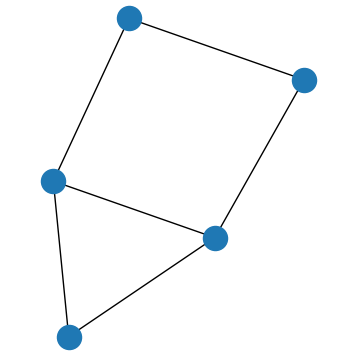
\includegraphics[width=0.2\textwidth]{figures/house.png} &
        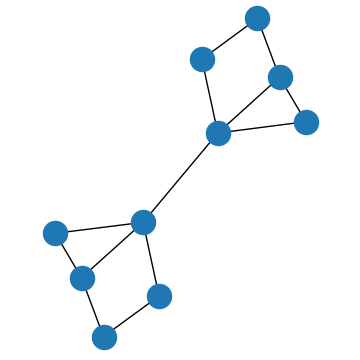
\includegraphics[width=0.2\textwidth]{figures/community.png} &
        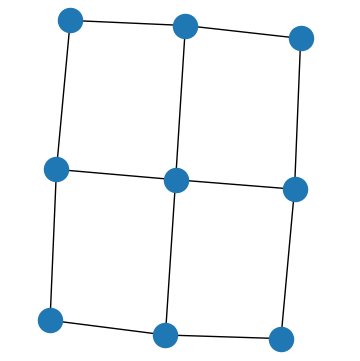
\includegraphics[width=0.2\textwidth]{figures/grid.png} &
        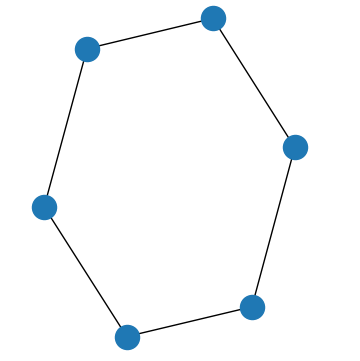
\includegraphics[width=0.2\textwidth]{figures/cycle.png} \\
    \end{tabular}
    \caption{The four different motifs used by the synthetic datasets. Each motif is attached to a specific base graph. Note that the community motif is created by combining two different shape motif graphs.}
    \label{tab:motifs}
\end{table}


are highly ordered graph structures that are easy to identify and differ from the structure of the base graph.
The four motifs can be seen in figure \ref{tab:motifs}.
As these motifs are also very simple they speed up the intensive process of calculating concept purity.

The following two graphs are used as base graphs:

\paragraph{Barabasi-Albert (BA)}
a densely connected graph where nodes are probabilisitically connected to each other.
The probability of a node connecting to another depends on the existing degree of the node thus keeping limiting the maximum degree of a node in the graph.

\paragraph{Tree}
a binary symmetric tree of height 8 and is therefore very sparse in comparison to Barabasi.
These two base graphs provide two different scenarios to compare a models ability to identify the motifs accurately.

Not all motifs and base graphs are paired together and only BA-Shapes\footnote{Which utilises the house motif}, BA-Grid, Tree-Grid and Tree-Cycles are considered.
There is an additional synthetic dataset, BA-Community, which combines two BA-Shapes graphs and requires the model distinguish between the communities as well as identify the motifs.

Node features for all the graphs are all-$1$ vectors of length 10, except in the case of BA-Community where one of the communities has all-$2$ vectors of length 10.

\subsection{Real-world datasets}
\label{sec:RWD}

% Linking to motivation and GRL
% Demonstrating that these techniques are important for real world use
% Discussions of the short comings of this approach

\textit{Wu et al.}\cite{wu2019simplifying} evaluate the performance of SGC on a variety of datasets including Cora, Citeseer and PubMed\cite{citation}.
These three datasets match the size of the datasets that are used in \textit{Magister et al.} and therefore are used for results reproduction.
Each graph represents a citation network where nodes are articles and edges are citations.
The node features are bag of word embeddings of the article abstracts or the entire article.
\note{Better description of the citation networks}
These datasets are available through \texttt{PyTorch Geometric}\cite{Fey/Lenssen/2019} under the Planetoid\cite{planetoid} datasets.

As an extension and to produce meaningful results that reflect real-world applications of GNNs two real world datasets are also tested against.
These two datasets are graph classification datasets and therefore inductive datasets compared to the transductive synthetic datasets.
These datasets are part of TUDataset \cite{Morris+2020} available through \texttt{PyTorch Geometric}\cite{Fey/Lenssen/2019}.

\paragraph{REDDIT BINARY}
is a dataset where each graph represents a discussion on Reddit with nodes being users and an edge represents one user responding to anothers comment.
The discussions are sampled from IAmA, AskReddit, TrollXChromosomes, and atheism.
IAmA and AskReddit are question-answer based whereas TrollXChromosomes and atheism are discussion based.
The task is to classify the graphs as question-answer or discussion based.

\paragraph{Mutagenicity}
is a dataset where each graph is a chemical compound where nodes are atoms and edges are chemical bonds.
The chemical compounds correspond to drugs some of which are mutagens and the rest are not.
The task is to classify the graphs as to whether or not they are mutagens.

\section{Tools used}

% I believe this is stuff like vim
% Pytorch, pytorch lightning and pytorch geometric
% scipy and numpy
% python unittest and typing
% python linter through vim

\paragraph{Programming languages}
I use Python to write the majority of the software as there is a lot of existing support for machine learning frameworks.
Furthermore, Python is easy to read, debug and iterate in which is very useful for developing and testing new methods.

To reduce the need for human input when running multiple experiments to get confidence intervals or hyperparameter tuning I also use bash scripts.
And to allow for easier reproducibility and iteration I utilise YAML files to store build configurations for all of my models.

\paragraph{Software development}

I use \texttt{NeoVim} to develop my code as this has high customisability allowing me to include specific linters to highlight bugs, typing errors and general static code analysis.
Additionally I use a local \texttt{Tensorboard} instance to visualise and analyse progress of my experiments in realtime, \texttt{Git} and \texttt{Github} for version control with \texttt{scp} and the \texttt{Student Run Computing Facility} as a third backup of experiment results.
I occasionally used \texttt{Google Colab} for compute units to run the large experiment batches.

\paragraph{Libraries}
\label{sec:libraries}

The major libraries I used where the two ML libraries \texttt{PyTorch} \cite{paszke2019pytorch} and \texttt{PyTorch Geometric} \cite{Fey/Lenssen/2019} an extension to \texttt{PyTorch} which includes support for GRL.
\texttt{PyTorch} was chosen over Tensorflow as it is more ``pythonic'' and \texttt{PyTorch Geometric} is a simpler framework to use.
To help with running experiments, logging results and reproducibility I use \texttt{Lightning AI} which handles the underlying training and testing loop while integrating with Tensorboard.
\texttt{Hyperopt} is also used as \textit{Wu et al.}\cite{wu2019simplifying} state this method was used to find the weight decay hyperparameter.

For scientific computing when analysing concepts I use \texttt{Numpy} and \texttt{scikit-learn}. For the visualisation of graphs I use \texttt{NetworkX} to draw the graphs and \texttt{Matplotlib} to visualise and store the result, I also use \texttt{Matplotlib} to visualise hyperparameter surfaces. Note that \texttt{NetworkX} is included in the \texttt{PyTorch Geometric} library automatically.

For unit tests I use Python's own \texttt{unittest} library, to help with software development I use Python's \texttt{typing} library alongside the built in typing functionality of the other libraries. Additionally I use \texttt{tqdm} to visualise progress during concept analysis.

\section{Requirements analysis}

% definitely think this is useful
% to be figured out later

The success criteria of the project proposal (\Aref{ch:proposal}) three main stages of development each requiring individual and joint requirements.
Furthermore there are additional requirements to improve reproducibility of the code and desirable requirements for extensions.

Table \ref{tab:requirements} demonstrates the requirements analysis for this project.
Risk represents how critical a requirements success is given how difficult it will be to implement.

``-'' represents a general requirement for the project to be implemented, ``S'' represents a requirement based on the given success criteria, and ``E'' represents a requirement that is an extension to the core project.

\begin{table}
    \centering
    \begin{tabular}{p{0.11\textwidth}|p{0.5\textwidth}|p{0.15\textwidth}|p{0.11\textwidth}}
        \multicolumn{1}{c}{\textbf{Source}} &
        \multicolumn{1}{c}{\textbf{Requirement}} &
        \multicolumn{1}{c}{\textbf{Importance}} &
        \multicolumn{1}{c}{\textbf{Risk}} \\ 
        \midrule
        - & Download Planetoid and TUDatasets & \hlc[red!50]{Essential} & \hlc[green!50]{Low} \\
        - & Build synthetic datasets & \hlc[red!50]{Essential} & \hlc[red!50]{High} \\
        - & Implement ML pipeline & \hlc[red!50]{Essential} & \hlc[orange!50]{Medium} \\
        - & Create model configuration format & \hlc[orange!50]{Preferrable} & \hlc[green!50]{Low} \\
        S1 & Implementation of SGC & \hlc[red!50]{Essential} & \hlc[orange!50]{Medium} \\
        S1 & Implement Hyperparameter sweep framework & \hlc[orange!50]{Preferrable} & \hlc[green!50]{Low} \\
        S1 & Hyperparameter sweep for SGC\tablefootnote{GCN hyperparameters should be sufficient for a well performing SGC model, but for true comparison a full sweep of reasonable parameters should be made.} & \hlc[orange!50]{Preferrable} & \hlc[green!50]{Low} \\
        S2 & Implementation of GCN & \hlc[red!50]{Essential} & \hlc[green!50]{Low} \\
        S1, S2 & Match prior performance & \hlc[red!50]{Essential} & \hlc[red!50]{High} \\
        S1, S2 & Implement model hooks to extract activation space & \hlc[red!50]{Essential} & \hlc[green!50]{Low} \\
        S1, S2 & Implement clustering for concept extraction & \hlc[red!50]{Essential} & \hlc[green!50]{Low} \\
        S3 & Implementation of concept purity & \hlc[red!50]{Essential} & \hlc[green!50]{Low} \\
        S3 & Implementation of concept completeness & \hlc[red!50]{Essential} & \hlc[orange!50]{Medium} \\
        S1, S2, S3 & Concept visualisation & \hlc[orange!50]{Preferrable} & \hlc[green!50]{Low} \\
        E & Extend SGC to graph classification & \hlc[green!50]{Optional} & \hlc[orange!50]{Medium} \\
        E & Improve performance of SGC & \hlc[green!50]{Optional} & \hlc[gray!50]{Unknown} \\
        E & Combine SGC and GCN & \hlc[green!50]{Optional} & \hlc[gray!50]{Unknown} \\
        E & Latent space comparison of GCN and SGC & \hlc[green!50]{Optional} & \hlc[gray!50]{Unknown} \\
    \end{tabular}
    \caption{Requirements analysis for the project.}
    \label{tab:requirements}
\end{table}

%\begin{enumerate}
%    \item[S1] Implementation of SGC
%    \item[S2] Implementation of GCN
%    \item[S3] Implementation of concept evaluation
%\end{enumerate}



\section{Software methodology}

% Generally waterfall approach to design
% But iterative when looking at the results and direction forward
% sprint work style between meetings

For the core of my project I adopt a Waterfall method \cite{royce1970managing} for my project:

\begin{equation*}
    \textit{Requirements analysis} \longrightarrow \textit{Design} \longrightarrow \textit{Implementation} \longrightarrow \textit{Testing} \longrightarrow \textit{Evaluation}
\end{equation*}

During the \textit{Design} phase I start with a skeleton implementation of the ML pipeline and focus on each of the requirements in turn carrying out both \texttt{Implementation} and \texttt{Testing} together where possible.
At each stage I confirm that the implemented requirement integrates with the rest of the project using a combination of predetermined dummy data, dummy models and dummy concept analysis where these aspects where not yet implemented.
\textit{Evaluation} stage includes all the experiment runs and concept analysis required to meet my success criteria replacing \textit{Operations} which is not required for my project.

My extensions do not fit into the Waterfall method as they are research based in nature. I therefore switch to an Agile software development \cite{beck2001manifesto} to allow the project to adjust to the experimental results achieved during development.

\section{Testing}
\label{sec:testing}

% unittest for specific sections of code and infrastructure
% comparison to paper baselines when dealing with model implementation

Machine learning does not provide precise metric against which correctness of an implementation can be verified.
This is due to the multiple factors that contribute to a machine learning models performance such as hyperparameters, initialisation/random seeds, architecture and dataset.
As example a trained model may result in poor results because the underlying architecture is not suited to the dataset, there is too much noise in the data to properly train, or because there is a software bug.
Thus, unlike traditional software development, it is much harder to verify that an ML model or algorithm has been implemented correctly.
However, my project does include software that follows traditional software development and therefore a use the following two testing approaches:

\paragraph{Unit testing}
is suitable for traditional software development where a specific result is required for specific input.
The concept analysis and dataset handling fall into this category.
These two aspects are therefore verified using unit testing described in \Sref{sec:testing-imp}.

\paragraph{Reproduction of prior results}
The two main models I use, GCN and SGC, directly follow implementations of the work by \textit{Kipf et al.}\cite{kipf2016semi} and \textit{Wu et al.}\cite{wu2019simplifying}.
The hyperparameters for the GCN model baseline are available in \textit{Magister et al.}\cite{magister2021gcexplainer} where accuracy scores are also published.
In \Sref{sec:reproduction} I reproduce the experiment results to verify my ML pipeline, NN implementations and dataset integration.

\section{Licensing}
%%\begin{table}
    \centering
    \begin{tabular}{cc}
        \multicolumn{1}{c}{\textbf{Software dependency}} &
        \multicolumn{1}{c}{\textbf{License}} \\ 
        \midrule
        NumPy & \multirow{5}{*}{3-clause BSD} \\
        scikit-learn & \\
        NetworkX & \\
        PyTorch & \\
        hyperopt \tablefootnote{The license is unnamed but matches the 3-clause BSD license verbatim.} & \\
        \rowcolor{gray!20} tensorboard & \\
        \rowcolor{gray!20} Lightning AI &  \multirow{-2}{*}{Apache 2.0}\\
        matplotlib & \\
        Python & \multirow{-2}{*}{PSFL}\\
        \rowcolor{gray!20}
        PyTorch Geometric & \\
        \rowcolor{gray!20}
        tqdm & \multirow{-2}{*}{MIT} \\
        tqdm & MPL\tablefootnote{tqdm is distributed under both licenses.} \\
    \end{tabular}
    \caption{Licenses for the project dependencies}
    \label{tab:licensing}
\end{table}

\begin{table}
    \centering
    \begin{tabular}{cc}
        \multicolumn{1}{c}{\textbf{Software dependency}} &
        \multicolumn{1}{c}{\textbf{License}} \\ 
        \midrule
        NumPy & \multirow{5}{*}{3-clause BSD} \\
        scikit-learn & \\
        NetworkX & \\
        PyTorch & \\
        hyperopt \tablefootnote{The license is unnamed but matches the 3-clause BSD license verbatim.} & \\
        \rowcolor{gray!20} tensorboard & \\
        \rowcolor{gray!20} Lightning AI &  \multirow{-2}{*}{Apache 2.0}\\
        matplotlib & \\
        Python & \multirow{-2}{*}{PSFL}\\
        \rowcolor{gray!20}
        PyTorch Geometric & \\
        \rowcolor{gray!20}
        tqdm & \multirow{-2}{*}{MIT} \\
        tqdm & MPL\tablefootnote{tqdm is distributed under both licenses.} \\
    \end{tabular}
    \caption{Licenses for the project dependencies}
    \label{tab:licensing}
\end{table}

Table \ref{tab:licensing} includes information about the specific licenses for all the software dependencies in my project.

All software dependencies used in my project are under permissive licenses allowing me to use the code with no restrictions.
Furthermore, I am free to use the Planetoid \cite{planetoid} and TUDataset \cite{Morris+2020} datasets available in \texttt{PyTorch Geometric} library.
Though some licenses have additional restrictions on source code modification and/or redistribution my project does neither of these actions and only uses the libraries as is.

I license my source code under the MIT license to support further developers and researchers.
This licensing complies with the licenses of my dependencies.

% Definitely need to research this aspect

\section{Starting point}

My starting point is the same as the starting point declared in my proposal except for the additional information that the research paper over the summer has resulted in an acceptance to Learning on Graphs 2022.
I use the \texttt{PyTorch Geometric} implementation of GCN layers to build the GCN network, as this is just a baseline model. I also rely on the libraries discussed in \Sref{sec:libraries}.
Aside from these dependencies I built the project from scratch.

% Discussion of summer project using the same rough build environment
